% CFP: https://www.usenix.org/conference/atc20/call-for-papers
\documentclass[letterpaper,twocolumn,10pt]{article}
\usepackage{usenix2019_v3}

\usepackage{soul}
\usepackage{xspace}
\usepackage{color}
\usepackage{booktabs}
\usepackage{graphicx}
\usepackage{alltt}
\usepackage{amssymb}
\usepackage{amsmath}
\usepackage{listings}

\lstdefinelanguage{js}{
  morekeywords={typeof, let, new, true, false, catch, function, return, null, catch, switch, var, if, in, while, do, else, case, break},
  keywordstyle=\color{purple}\ttfamily,
  keywordstyle=[3]\color{orange},
  keywords=[3]{SBX, PROC},
  ndkeywords={class, export, require, boolean, throw, implements, import, this},
  ndkeywordstyle=\color{cyan}\ttfamily, %bfseries
  identifierstyle=\color{black},
  sensitive=false,
  comment=[l]{//},
  commentstyle=\color{lightgray},
% morecomment=[s]{/\\*\\*, \\*/},
  stringstyle=\color{blue}\ttfamily,
  basicstyle=\footnotesize\ttfamily,  % the size of the fonts that are used for the code
  numberstyle=\tiny\color{gray},   % the style that is used for the line-numbers
  morestring=[b]',
  morestring=[b]",
% moredelim=[s][\color{gray}]{c:}{>},
% moredelim=[s][\color{orange}]{/*}{/}
}

\lstdefinelanguage{es}{
  morekeywords={string, number, bool, p, v, e, x},
  keywordstyle=\color{darkgray},
  keywordstyle=[3]\color{orange},
  keywords=[3]{SBX, PROC},
  ndkeywords={undefined, null, delete},
  ndkeywordstyle=\color{black}\ttfamily\bfseries,
  identifierstyle=\color{black},
  sensitive=false,
  comment=[l]{//},
  commentstyle=\color{lightgray},
% morecomment=[s]{/\\*\\*, \\*/},
  stringstyle=\color{darkgray}\ttfamily,
  morestring=[b]',
  morestring=[b]",
% numbersep=1pt,
% numberstyle=\footnotesize\bf\color{gray},   % the style that is used for the line-numbers
  abovecaptionskip=0em,
  aboveskip=0em,
  belowcaptionskip=0em,
  belowskip=0em,
  frame=none,                     % adds a frame around the code
% moredelim=[s][\color{gray}]{c:}{>},
% moredelim=[s][\color{orange}]{/*}{/}
}

\lstset{ %
  backgroundcolor=\color{white},   % choose the background color; you must add \usepackage{color} or \usepackage{xcolor}
  basicstyle=\small\ttfamily,  % the size of the fonts that are used for the code
  upquote=true,
  captionpos=b,                    % sets the caption-position to bottom
% frame=B,                    % adds a frame around the code
  numbers=left,                    % where to put the line-numbers; possible values are (none, left, right)
  numbersep=3pt,                   % how far the line-numbers are from the code
  numberstyle=\tiny\color{gray},   % the style that is used for the line-numbers
  rulecolor=\color{black},         % if not set, the frame-color may be changed on line-breaks within not-black text (e.g. comments (green here))
}


\usepackage{caption}
\captionsetup[figure]{font=footnotesize,name={Fig.},labelfont={bf, footnotesize}}
\captionsetup[table]{font=footnotesize,name={Tab.},labelfont={bf, footnotesize}, skip=2pt, aboveskip=2pt}
\captionsetup{font=footnotesize,labelfont={bf, footnotesize}, belowskip=2pt}

\usepackage{enumitem}
\setlist{noitemsep,leftmargin=10pt,topsep=2pt,parsep=2pt,partopsep=2pt}

\def\omit#1{}
\def\eg{{\em e.g.}, }
\def\ie{{\em i.e.}, }
\def\etc{{\em etc.}\xspace}
\def\vs{{\em vs.}\xspace}
% \newcommand{\heading}[1]{\vspace{4pt}\noindent\textbf{#1}\enspace}
% No vspace, coz Usenix class already has paragraph space
\newcommand{\heading}[1]{\vspace{2pt}\noindent\textbf{#1}\enspace}
\newcommand{\ttt}[1]{\texttt{#1}}
\newcommand{\ttiny}[1]{\texttt{\footnotesize #1}}
\newcommand{\tcn}[1]{}

\definecolor{cdb}{rgb}{0.37, 0.62, 0.63} % cadet blue

\newcommand{\cf}[1]{(\emph{Cf}.\S\ref{#1})}
\newcommand{\sx}[1]{(\S\ref{#1})}
\newcommand{\tb}[1]{(Tab.\ref{tab:#1})}
\newcommand{\rf}[1]{\ref{#1}}
\newcommand{\se}[1]{\S\ref{#1}}
\newcommand{\fg}[1]{Fig.~\ref{#1}}

\newcommand{\sys}{{\scshape Lya}\xspace}
\newcommand{\toy}{{\tt lya.js}\xspace}


\newcommand{\fra}{fracture\xspace} % fracture?
\newcommand{\ana}{analysis\xspace}      % 
\newcommand{\ass}{reassembly\xspace}    % 
\newcommand{\Fra}{Fracture\xspace} % fracture?
\newcommand{\Ana}{Analysis\xspace}      % 
\newcommand{\Ass}{Reassembly\xspace}    % 
\newcommand{\dia}{\fra, \ana, and \ass}

\newcommand{\R}{\ttt{R}\xspace}
\newcommand{\W}{\ttt{W}\xspace}
\newcommand{\X}{\ttt{X}\xspace}
\newcommand{\E}{\ttt{X}\xspace}
\newcommand{\rwx}{\ttt{RWX}\xspace}

% FIXME:
\newcommand{\pc}{PIC\xspace}
\newcommand{\pcs}{\pc{}s\xspace}

\newcommand{\goal}[1]{(\textbf{G#1})\xspace}

\newcommand{\nv}[1]{[{\color{cyan}#1 --- Nikos}]}
\newcommand{\review}[1]{{\color{red}#1}}
\newcommand{\TODO}[1]{\hl{\textbf{TODO:} #1}\xspace}
\newcommand{\todo}[1]{\hl{#1}\xspace}
\newcommand{\fixme}[1]{{\color{red}#1}}
\newcommand{\tc}{(\todo{cite})\xspace}
%-------------------------------------------------------------------------------
\begin{document}
%-------------------------------------------------------------------------------

\date{}

\title{\Large \bf \sys: Library-Oriented Program Analysis}

\author{
% {\rm Anonymous Author(s)}\\
% \normalsize{Additional Anonymized Material: \href{https://git.io/JvfCf}{https://git.io/JvfCf}.}
% {\rm Nikos Vasilakis \quad Grigorios Ntousakis\textsuperscript{$*$} \quad Martin Rinard}\\
% MIT, CSAIL \quad \quad \quad \textsuperscript{$*$}TU Crete, ECE
}

\maketitle

\begin{abstract}

Dynamic program analysis is a long-standing technique for obtaining information about program execution.
We present a new dynamic analysis approach that targets modern dynamic languages such as Python, Lua, and JavaScript, enabled by the fact that they feature a module-import mechanism that loads code at runtime as a string.
This approach uses lightweight load-time code transformations that operate on the string representation of the module, as well as the context to which it is about to be bound, to insert developer-provided, analysis-specific code into the module before it is loaded.
This code implements the dynamic analysis, enabling this approach to capture all interactions around the library in unmodified production language runtime environments.
We implement this approach in \sys, a system targeting the JavaScript ecosystem. 
Results show that \sys delivers over an order of magnitude performance improvements over current state-of-the-art dynamic analysis systems, compatibility with over 50 libraries and applications, and support for a range of dynamic analyses, each implemented in under 100 lines of code.
\end{abstract}

\section{Introduction}
\label{intro}

Dynamic analysis is a type of analysis performed by (and while) executing a program, with the goal of extracting information about the program and its execution.
Such information may include the ability to infer execution invariants, check security constraints, and extract performance characteristics~\cite{analysis:10}.
Contrary to other types of analysis, its key benefits make it the primary (or only) candidate in a variety of scenarios---namely, ones that require:
  (i) current runtime information, such as profiling data, in view of changing load patterns~\cite{staticdynamic},
  (ii) accurate visibility into the execution, devoid of imprecision or approximation~\cite{staticdynamic},
  (iii) Turing-complete policies, where monitors themselves are programs~\cite{contracts1, contracts2, contracts3},
  (iv) dynamic or runtime-reflection features, such as the ones present in Python and JavaScript~\cite{jsanalysis1, jsanalysis2}.

Unfortunately, reaping these benefits comes with significant costs in terms of developer effort or runtime performance.
Manually instrumenting a program requires a good understanding of its internals. 
External tools such as instrumentation frameworks~\cite{pin, valgrind} and performance tracing tools~\cite{perf, dtrace} only add to the curve, as they feature their own language for specifying analyses. 
Modifying the application's runtime environment such as the interpreter is cumbersome, error-prone, and requires development in a language that is different than that of the program.
Tools that virtualize execution~\cite{pin, valgrind, jalangi, roadrunner} have high performance costs---for example, Jalangi~\cite{jalangi} and RoadRunner~\cite{roadrunner} report No-Op analysis on the order of 26--32$\times$ and 52$\times$, respectively.
% Problem-specific solutions require significant investment outside the language's mental model---for example,  each ---as a case in point, Jalangi reports XX overhed (exact overheads always depend on the specific analysis).

Effort and performance costs are severely compounded by the use of third-party libraries,\footnote{
  The terms library, package, and module are used interchangeably.
}
often glued together without full understanding of their internals~\cite{libs}.
% This is a recent phenomenon enabled by zero-cost code sharing
%   language-specific package repositories eliminate the cost of publishing and using a library.
Applications frequently count hundreds of libraries~\cite{npmstudy:19}, each one often only a few lines long~\cite{leftpad, npmstudy:19}. % how to say thousands of them depend on a 11-line lib?
Library-oriented analysis adds to the challenges of prior tools as
  (i) library boundaries disappear at runtime, and
  (ii) coarse-grained, high-level language semantics misalign with fine-grained, low-level instrumentation.

This paper presents a novel approach to dynamic analysis, targeting dynamic programming languages---and implemented in \sys for the server-side JavaScript ecosystem (>1.3M libraries~\cite{modulecounts}). 
\sys leverages the ability of these languages to import code at runtime as a string in order to apply transformations that wrap the module about to be imported with developer-provided, analysis-specific code.
More specifically, \sys inserts a series of steps in the module-loading process result in wrapping a library's full observable behavior---rather than just its interface---and exposing it to developers for runtime analysis.
\sys effectively fragments, transforms, and reassembles the application at the level of individual libraries. 
The overall approach has several practical benefits over prior work:
  (i) it allows bolting the dynamic analysis as a library  onto unmodified runtime environments,
  (ii) it supports analyses expressed using the same language, tools, and abstractions as the program language,
  (iii) it features low runtime performance overheads, enabling toggling its use in production environments.

% \heading{Is it Useful?}
% First question
% 
% \heading{Is it Usable?}
% Example 
% 
% \heading{Is it Performant?}
% Highlight results

To demonstrate that \sys can be useful in practice, despite its coarse granularity, we develop a diverse set of analyses:
  a read-write-execute security analysis,
  a profiling analysis for identifying bottlenecked modules,
  and an analysis extracting union-based type invariants.
% These analyses drive \sys's design requirements, and highlight the decisions behind its design.
Each of these analyses takes about 100 LoC in JavaScript;
  this integration between the code being analyzed and the one implementing the analysis has significant usability implications.
Finally, \sys's performance is evaluated extensively, using
  (i) over 50 popular libraries and scripts, highlighting compatibility and performance improvements over state-of-the-art frameworks;
  (ii) three full applications, demonstrating that \sys scales to large and complex programs; and
  (iii) a series of micro-benchmarks that zoom into a few specific characteristics of \sys.
\S\ref{bg}--\ref{eval} present our key contributions:
\begin{itemize}
\item \S\ref{bg} characterizes the shared needs of three case-study multi-module analyses whose needs remain mostly by general-purpose analysis frameworks.
\item \S\ref{design} presents the design of \sys, bolt-on library-oriented dynamic analysis, which meets the requirements of the three case-study analyses.
\item \S\ref{impl} discusses our implementation, \sys, as a pluggable library for the JavaScript ecosystem, as well as the implementation of the three analyses.
\item \S\ref{eval} evaluates \sys, showing that it expresses insightful analyses succinctly, adds minimal overheads over the baseline runtime, and scales to hundred-library programs.
\end{itemize}
\noindent
The paper then discusses \sys's limitations and its application to other languages~\sx{diss};
  it compares with related prior work~\sx{rw};
  and draws appropriate conclusions~\sx{end}.

\section{Background, Examples, and Goals}
\label{bg}

A single application today often incorporates multiple libraries written and published by several different authors.
To make the difficulties of analyzing such library-overreliant software more concrete, we describe three example analyses~\sx{examples}.
These examples illustrate key requirements for the design of a framework for analyzing applications at the boundaries of modules~\sx{goals}.
Before describing these examples, however, we offer a brief refresher on the %abstractions and corresponding
  internals of a module system~\sx{bg1}.

\subsection{Background on Module Systems}
\label{bg1}

\begin{figure}[t]
\raggedleft 
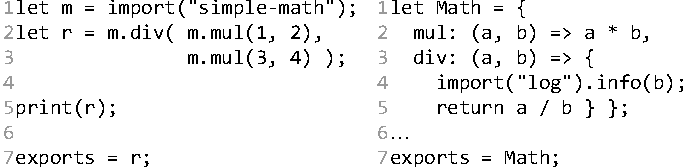
\includegraphics[width=0.45\textwidth]{./figs/lya_ex1.pdf}
\caption{
  \textbf{Example of a library import.}
  \textmd{
    The program on the left imports the \ttt{simple-math} library, shown right, which imports \ttt{log} and exports a \ttt{Math} object.
    Several names are provided by the programming language:
      \ttt{import} and \ttt{exports} resolve to library-local values; \ttt{print} resolves to a global value.
  }
  \vspace{-8mm}
}
\label{fig:ex1}
\end{figure}


Libraries are development-time construct encapsulating reusable functionality.
This functionality falls into two categories:
  it either (i) comes bundled with the language, possibly wrapping operating-system interfaces, such as the file-system, in a way that is system-agnostic and conforms to the language's conventions,
  or (ii) is provided by other developers sharing code others might find useful.
Fig.~\ref{fig:ex1} shows a \ttt{simple-math} library (right) imported by a program (left).

From a developer's perspective, \ttt{import}ing a library makes its functionality available to the calling code by means of binding its functionality to a name in the caller's scope.
This is achieved by some form of \ttt{export}ing, where the library developer expresses which values should become available to the \ttt{import}ing code.
The definition of a value depends on the semantics of the language. 
Internally, the library may \ttt{import} other libraries, cause side-effects to the file-system or the network, or even be implemented in multiple languages.

From the programming language's perspective, the process of \ttt{import}ing a library is achieved in several steps. 
Compiled languages support separate compilation, where source files are compiled individually, followed by a runtime-linking phase that loads and links the resulting object files.
Interpreted languages involve a somewhat convoluted process that combines runtime loading, interpretation, and linking.
This process starts by locating the library in the file system,
% or across the network,\footnote{
%   Examples of run-time environments featuring network loading include V8 and deno, for executing JavaScript and TypeScript respectively.
% }
by resolving code-relative module identifiers.
The content of the library is then read and wrapped in a way that resolves library-local names, such as \ttt{\_\_name\_\_} in Python and \ttt{\_\_filename} in JavaScript, to meaningful values.
The wrapper is then interpreted and evaluated using the language's interpreter, which might result in side-effects---for example, a \ttt{process.exit()} in the library's top-level scope will exit the entire program.
Finally, the value bound to the \ttt{export}ed interface or returned from this interpretation (depending on the language) is made available to the scope of the  \ttt{import}ing code.

There is significant variation, but a few features are common across many implementations.
A library cache maintains a mapping from library identifiers, often absolute paths, to returned \ttt{export} values.
The cache serves a dual purpose:
  by avoiding locating already loaded libraries, it improves performance and ensures the consistency of any library-internal state.
Recursive imports are handled in a depth-first way, and when cyclical dependencies are possible, they are resolved by pointing to the cache.
An increasingly common feature is to allow different versions of the same library to co-exist in a program, in order to avoid a choice between mutually exclusive options---a paradoxical situation known as ``dependency hell''.
As a result, a single \ttt{import} $l$ does not necessarily resolve to the same (version of the) library $l$ every time.
The dual of this is also possible:
   two different library names may resolve to the same identifier (\ie point to the same cache entry).
These features complicate library-level analysis, especially in interpreted programming languages.


\subsection{Motivating Examples}
\label{examples}

% Could add several details:
%   same module at multiple levels, and the module cache
%   sometime it's the same, some times it;s not
%   module resolution algorithm

Having reviewed the building blocks and underlying techniques that power modularity, we now turn to examples of dynamic analysis that today are difficult or require specialized solutions:
  (i) a read-write-execute security analysis,
  (ii) a performance-profiling analysis, and %  for identifying bottlenecked libraries, and
  (iii) an analysis extracting runtime type invariants.
These examples illustrate key design requirements for \sys.

\heading{Security Analysis}
The pervasive reliance on third-party libraries has led to an explosion of supply-chain attacks~\cite{long2015owasp, maass2016theory, snyk, lauinger2017thou}.
Both bugs and malicious code in libraries create attack vectors, exploitable long after libraries reach their end-users.
As library boundaries disappear at runtime, libraries end up executing with no meaningful isolation or privilege separation guarantees between each other and the trusted portions of a program.
Popular libraries, depended upon by tens of thousands of other libraries or applications, allow vulnerabilities deep in the dependency graph to affect a great number of applications~\cite{leftpad, npmstudy:19}.
Discovered vulnerabilities are becoming harder to eradicate, as updates are fetched automatically~\cite{npmFailure} and module unpublishing is becoming a multi-step process to avoid breaking applications~\cite{npmUnpublish}.
Worst of all, leaked publishing tokens allow attackers to update packages with code that will eventually reach end-users via package updates~\cite{eslint1}.

As a concrete example, consider the recent \ttt{event-stream} incident~\cite{es1, es2}, in which a maintainer of a highly popular library inserted code stealing Bitcoin wallet credentials from programs using that library.
Heavy-weight runtime instrumentation~\cite{jalangi} would not have helped, as \ttt{event-stream} activated only on production (rather than testing or development).
Coarse-grained analysis at program boundaries, say via containment or system-call interposition~\cite{systrace:03}, would have not helped either as the programs importing \ttt{event-stream} already made use of system calls to access the disk and network.
Finally, static analysis would have been of little use, as \ttt{event-stream} encrypted its malicious payload.

Having the ability to toggle a library-level ``allow-deny'' security analysis on/off at runtime would have revealed the (unusual) resources touched by \ttt{event-stream}.
Analyzing the behavior \emph{within} the library itself is not critical:
  if any data exfiltration is happening, it will require calling out of the library and into the network---in \ttt{event-stream}'s case, using the \ttt{fs} library to modify a different library and then call \ttt{http} from the second library.
Both \ttt{fs} and \ttt{http} are part of the standard library, built into the runtime environment.
Other examples of interfaces that are available to the entire program include global variables, library importing, and the module cache---all of which are accessible by any third-party library.
% The key issue underlying the \ttt{event-stream} attack is that any third-party fragment of an application has unrestricted access to the functionality available to the rest of application.

\heading{Performance Diagnosis}
Diagnosing performance problems is a difficult task, exacerbated by the heavy use of third-party libraries.
Libraries are written by authors with different education, backgrounds, quality standards, and, most importantly, needs:
  it is not unusual for a weekend project solving a local need to end up as a critical dependency among several open-source projects~\cite{cheapcomplexity}.
Maintenance and rewriting can also cause performance regressions between two versions of a library;
  worse even, the fact that a library changes one of its dependencies can cause severe performance pathologies to upstream projects---that is, while an interface remains the same due to an intermediate layer of abstraction, its performance can change dramatically~\cite{jest}.

As a concrete example, consider the \ttt{minimatch} library, a regular-expression-based file-matching utility susceptible to long delays due to regular expressions that involve backtracking~\cite{minimatch}.
Pathological inputs reaching \ttt{minimatch}, even if benign, can cause significant performance degradation~\cite{redos} deep in the dependency chain, affecting also other parts of the program competing for the same resources~\cite{evp}.
Developers use various techniques to understand such problems---\eg collecting and replaying traces against off-line versions of the system, or using statistical profiling to identify hot code-paths.
These techniques, however, require significant \emph{manual} effort:
  capturing traces, setting up test-beds, replaying traces, analyzing statistics, and debugging performance are all tedious and time-consuming tasks, compounded by the difficulties of mapping the results to the right third-party libraries.

Switching-on a library-level profiling analysis 
  would quickly detect a slowdown and attribute it to the bottlenecked \ttt{minimatch}.
Wrapping library interfaces with profiling logic can be of aid to constructing a model of the current workload.
Such profiling could operate at a high resolution in time and space---at every function call entering a library and on hundreds of libraries across an application---but does not need to track detailed operations such as direct variable accesses.
Each library wrapper can collect profiling statistics at its own boundary, aggregating summaries into a global structure ordering libraries by resource consumption.

\heading{Type Invariant Discovery}
Extracting type information in at the library boundary is helpful in a variety of scenarios. %, as type safety is an important property helpful in variety of scenarios. 
Types can be used to
  (i) identify library invariants to be preserved during code modifications,
  (ii) generate (machine-checkable) library documentation, or 
  (iii) guide library synthesis and regeneration~\cite{daikon}.
This is especially important in dynamic programming languages:
  in the absence of static type signatures, there is not much one can say about a library without executing it and inspecting its properties.

As a case in point, consider the \ttt{gRPC} library for serializing and de-serializing objects~\cite{grpc}.
To use it, developers have to provide a protocol-buffer specification describing the types of values that will be serialized.
Given a library---\eg \ttt{bignum}, \ttt{crypto}---a developer has to first call it manually, take note of the result's type, and then fill in the protobuf spec.
This process has to be repeated with every change, often due to library updates or changes in the consuming program's structure.

Library-level dynamic analysis can be used to discover such type assertions or invariants.
The analysis would consult the (static) definition of a type system, capturing the type of values at the boundaries of libraries by observing their arguments during the execution of the program.
%% TODO: such as the simply-typed lambda calculus augmented with objects and union types.

\subsection{Design Goals}
\label{goals}

We have briefly introduced three motivating analyses for extracting information about an application's dependencies.
While the challenges behind these analyses share several characteristics, today they remain largely unaddressed by dynamic analysis frameworks due to a combination of factors:
  these frameworks either require highly specialized solutions often outside the core language,
  do not leverage nor offer semantic information at the level of library boundaries, or
  lead to a high (often impractical) performance overheads due to the high granularity of their analyses.
To summarize, these applications would appear to be served well by a system that:
\begin{itemize}
  \item \textbf{(G1)} Operates at the level of libraries, leveraging both the semantics and performance potential that this level of granularity can potentially offer.
  \item \textbf{(G2)} Does not require learning a new tool or language, but rather allows developers to express their analyses in the same language as the program.
  \item \textbf{(G3)} Can be implemented as a library that bolts analyses onto an existing language runtime environment.
% \item \textbf{(G4)} It does not incur prohibitive overheads, such that it can be switched on and off selectively during runtime execution.
\end{itemize}

The next section describes the design of \sys, a new dynamic analysis framework that satisfies these goals, in a language-agnostic manner~\sx{design};
  the section following that describes \sys's concrete implementation for server-side JavaScript~\sx{impl}.

\section{The Design of \sys}
\label{design}

\sys starts by dynamically modifying the functionality of the module system that is responsible for importing and loading libraries:
  instead of simply locating and loading a library from the file-system, it yields control to \sys, which applies a series of transformations to libraries with the goal of interposing at their boundaries.
We start with an overview of \sys~\sx{overview}, highlighting several key challenges, followed by a detailed description of each step~(\S\ref{one}--\ref{three}).

\subsection{Overview}
\label{overview}

% FIXME: add user data
\sys operates by
  dismantling the program at the boundaries of libraries,
  applying transformations that insert analysis-specific machinery, and then carefully 
  reassembling individual components to maintain the original semantics:

\begin{itemize}
  
  \item \textbf{Fracture:}
\sys starts by recursively dismantling a program into its dependencies. % ---pieces of software implement a computation or functionality.
This is achieved by re-wiring the language's \ttt{import} function to go through \sys, resulting in \sys walking the program's recursive dependency structure at runtime.
During this phase, \sys has to determine the granularity of the analysis (\eg top-level libraries, a specific library \etc) in order to apply transformations at the correct level and map the provided analysis hooks to the corresponding libraries.

  \item \textbf{Transformation:}
It then sets up the provided analysis, by transforming each library interface, its surrounding environment, and possibly the values passing through the library boundary.
Programmatic transformations walk and wrap each one of these values based on their type.
% the library interface is usually a complex (but singular) object;
% the surrounding environment provides names to multiple ``implicitly'' imported libraries, functionality provided by the language.
This phase requires solving several challenges, including enumerating all points of entry into and exit out of a library, 
and swapping all original values externally-available to a library with ones that are wrapped with interposition mechanisms.

  \item \textbf{Reassembly}
Finally, \sys reassembles individual modified libraries back into the program's original structure.
The most important challenge during this phase is the treatment of the library cache~\sx{bg1}.
The cache needs to be augmented to support multiple wrappers per library, each capturing a part of the overall analysis.
% without breaking the program's semantics.
% ensure every fragment finds its place during dependency reassembly, 

\end{itemize}

\begin{figure}[t]
\raggedleft 
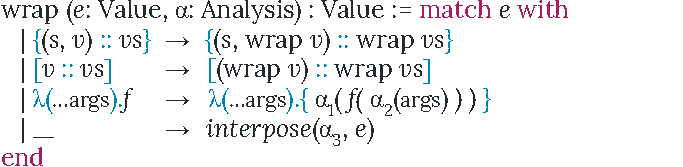
\includegraphics[width=0.45\textwidth]{./figs/lya_base.pdf}
\caption{
  \textbf{Base transformation.}
  \textmd{
  The algorithm (simplified) is presented in functional style to simplify variable binding; types (object, list, function, and primitive), used for pattern matching, are shown in light {\color{cdb} \emph{turquoise}}~\cf{two}. The functions $\alpha_1$, $\alpha_2$, and $\alpha_3$ stand for the locations of analysis hooks.
  }
  \vspace{-4mm}
}
\label{fig:base}
\end{figure}

\subsection{Fracture}
\label{one}

When a \sys-augmented program starts, it first loads the analysis file provided by the developer. 
The file may specify a subset of libraries whose boundaries are of interest or a subset of libraries that should \emph{not} be analyzed.
Among other things, \sys needs to determine the library boundaries of interest and the granularity of analysis.
To do this, it extracts an approximation of the dependency graph by traversing library files.
Using this graph, it processes the analysis file to extract a mapping from library identifiers to analysis hooks.
It also checks for constructs not associated with libraries---for example, whether the analysis includes global variables, library-local constructs, standard libraries \etc
\sys then proceeds to dynamically replace the implementation of \ttt{import} and launch the program:
  rather than simply locating and loading a library, calls to \ttt{import} now yield to \sys.

For every invocation of \ttt{import} \sys checks the cache~\sx{three} to determine
  (i) if the library has already been loaded, and
  (ii) whether it has been loaded with the same analysis hooks.
If both are determined true, \sys retrieves the cached version of the library and returns the transformed \ttt{export}ed value.
If the library was loaded with a different analysis---say because there are different analyses applied to different parts of a dependency tree---\sys constructs the appropriate analysis and applies a transformation pass on a cached copy of the unmodified library~\sx{three}.
Otherwise, \sys first invokes the built-in library loader to locate the library.

The process of loading new libraries includes (i) a phase of reading the necessary source files and (ii) a phase of interpreting them, interspersed by applications of transformations~\sx{two}.
Reading files returns a string representation of the code; interpretation uses the language's runtime evaluation primitives to convert the code into an in-memory object.

%FIXME: Need to start with both problems
Some analyses may themselves make use of global variables, libraries, and other analyzable constructs.
As these will be part of the same execution context, \sys must note to avoid transforming and wrapping these constructs as part of the analysis.
% The analysis language is embedded in the source language, thus \sys makes use of the language's built-in evaluation primitives to interpret the \pc specification file.
\sys frameworks may also want to add analysis-specific keywords not provided by the language.
To achieve this, \sys wraps each analysis hook with a function whose body starts by defining the expected keywords.
The precise techniques for achieving this will be made clear in the next section~\sx{two}, after covering transformations;
  the key point to remember is that analyses are initially represented as source strings, similar to libraries.

\begin{figure}[t]
\centering 
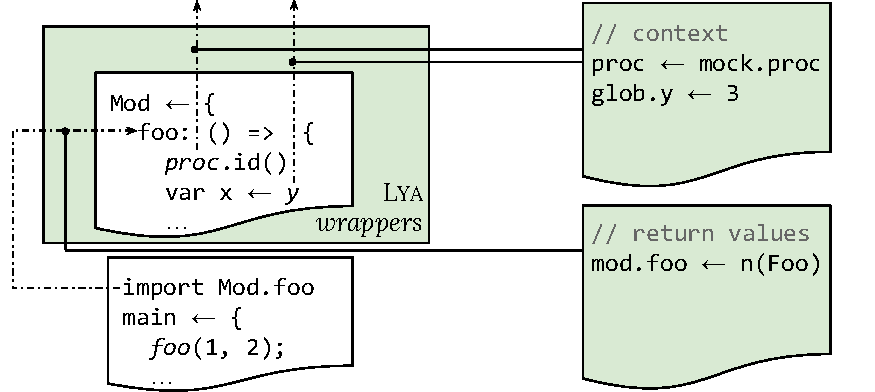
\includegraphics[width=0.45\textwidth]{./figs/lya_shadowing.pdf}
\caption{
  \textbf{Shadowing segments.}
  \textmd{
  Cross-module variable name resolution (left) augmented with \sys (green boxes), which interjects non-bypassable steps resolving to \sys-augmented values (right-top: implicit module imports; right-bottom: explicit import)~\cf{two}.
  }
  \vspace{-4mm}
}
\label{fig:shadowing}
\end{figure}


\subsection{Transformation}
\label{two}

%FIXME: Needs examples, especially the context
For each analyzed library, \sys needs to place hooks all around its boundary---not just its interface (Fig.~\ref{fig:shadowing}).
This is achieved in three logical steps:
(i) transforming the library's context, a mapping from names to values that are available from outside library,
(ii) interpreting the library within this context, so that all names bind and resolve to \sys-augmented values, and
(iii) transforming the library's \ttt{export} value, \ie the library interface, once the interpretation is complete.
Before discussing \emph{where} each transformation is applied, however, we show \emph{how} they are applied.

\heading{Transformations}
\sys's transformations boil down to a base transform \ttt{wrap} that traverses and augments values with runtime analysis monitors.
At a high level, \ttt{wrap} takes a value $v$ and analysis fragments $(\alpha_1, \alpha_2)$ and returns a new value $v'$ that has every one of its fields $f$ wrapped:
   every $f$ is replaced with a method $f'$ that calls fragment $\alpha_1$, calls $f$, calls fragments $\alpha_2$, and returns the result of the call to $f$.

More specifically, \ttt{wrap} can be applied to any value in the language, which can generally be a primitive, a function, or a compound value---say, a list of values or an object of key-value pairs.
% Listing~\ref{core-tx} presents a simplified core of the language.
Transformations walk compound values from their root, processing component values based on their types (Fig.~\ref{fig:base}):
% More specifically,
  (i) \emph{function} values are wrapped by closures that contain analysis-specific hooks; % on the function's arguments and return values;
  (ii) \emph{object} and \emph{list} values are recursively transformed, with their getter and setter methods replaced similar to function values; % and at times combining return results; and
  (iii) \emph{primitive} values are either transformed directly or copied unmodified and wrapped with an access interposition mechanism.
To avoid cycles during the walk, values are added to a map that is consulted at the beginning of each recursive call.

Direct field accesses, such as assignments, require detection upon access.
To achieve this, \sys wraps fields with an interposition mechanism;
  this mechanism essentially treats direct field accesses as function calls (see \S\ref{impl} for implementation details and \S\ref{reqs} for equivalents in other environments).
% Examples of such mechanisms include \ttt{Proxy} objects (JavaScript), metatables (Lua), metaclasses (Python), and direct-accessor metaprogramming (Ruby).
Extending a transformed object with a value will start with the value's transformation.
% \sys's wrappers detect and record changes to any of the object's fields, transforming values as needed.
For example, if a field in a transformed object is assigned a new value, that value has to be transformed before it is attached to the object.

\sys allows toggling analyses on/off, changing analyses, or chaining multiple analyses during the execution of the program.
To achieve this, it maintains a handle to the root of both the unprocessed and the newly processed values, for further processing:
  the unprocessed value is used to create objects, at runtime, that run different analyses;
  the new value is used to revoke or chain analyses together.

\heading{Context Transformation}
To be able to track an analysis at the library boundary, \sys needs to provide each library with values that are augmented with interposition wrappers---and do this for all of the names to which a library has access.
This includes global and pseudo-global\footnote{
  For example, Node introduces objects that are not part of the EcmaScript specification into the global scope, such as \ttiny{process} and \ttiny{console};
  similarly, Lua's Luvit introduces its own globals such as \ttiny{p()} and \ttiny{exports}.
} names provided by the language and its runtime.

To achieve this, \sys first needs to prepare a transformed copy of the library's context---a map from variable names that are (expected to be) in scope to their values.
\sys creates an auxiliary hash table mapping names to transformed values.
Names correspond to any name that, by the language definition, is accessible by the library and resolves to a value outside that library, such as globals, built-ins, module-locals, \etc
Transformed values are created by applying \ttt{wrap} to values in the context, adding the provided analysis hooks.

%% FIXME: 
%% While user-defined global variables are stored in well-known locations,\footnote{
%%   For example, \ttt{globals} in JavaScript and \ttt{\_G} in Lua.
%% } traversing the global scope for built-in values is generally not possible.
%% To solve this problem, \sys collects such values by resolving well-known names hard-coded in a list;
%%   different lists exist for different environments and versions of the language.
%% Using this list, \sys creates a list of pointers to unmodified values. % upon startup.

Care must be taken with library-local variables. % that refer to library-specific information such as \ttt{\_\_name\_\_} in Python~\sx{bg1}.
These are accessible from anywhere within the scope of a library (similar to global variables), but resolve to a different value for each library.
Examples include the library's absolute filename as \ttt{\_\_name\_\_}, its \ttt{export}ed values, and whether the library is invoked as the application's \ttt{main} library~\sx{bg1}.
Attempting to access library-local variables directly from within \sys's scope will fail subtly, as they will end up resolving to library-local values of \sys \emph{itself}---and specifically, the module within \sys that is applying the transformation.
\sys solves this problem by leaving the value empty and deferring binding for later from within the scope of the library (see below).

\heading{Context Binding}
To link the library with the newly transformed version of its context, \sys wraps the library---still an uninterpreted string of source code---with a closure.
The closure's body starts with a prologue of the form:
\begin{verbatim}
  local print = ctx.print
  local error = ctx.error
  ...
\end{verbatim}
These statements shadow global variable names by redefining them as function-local ones.
The closure accepts an argument \ttt{ctx} that will hold the customized context (see above), assigning its entries to their respective variable names.
The prologue executes before everything else in the library.
This technique leverages lexical scoping to inject a non-bypassable step in the variable name resolution process:
  instead of resolving to variables in the context, resolution will first ``hit'' library-local values augmented with analysis monitors.

Late-bound, \emph{library}-local variables, such as the absolute filename mentioned during context creation, are the result of applying \ttt{wrap} over variable names in the current scope;
  these names are now bound to the correct library-local values.

\heading{Library Interface Transformation}
Returning the library's value to its consumer amounts to interpreting the library, linking it with the custom context, and applying a final transformation to its return value.
% TODO: (for intro!) ..to attenuate the privilege exercised by the library's consumer
The goal of the final transformation is to track activity at the boundary.\footnote{
  For some analyses, \sys needs to additionally augment the values going through the library's interface---including continuation functions passed as arguments to the library's methods.}
This final transformation is applied for every new consumer of the library, returning a fresh analysis wrapper.
This is due to the need for distinguishing between different boundaries of the same library.

The treatment of this feature during reassembly is explained in the next section~\sx{three}.
  

\subsection{Reassembly}
\label{three}

To successfully reassemble the application, \sys needs to ensure that cross-references between libraries resolve correctly.
The central mechanism for this resolution is the library cache.

To support multiple wrappers for a single cached library, the cache is extended by two levels (for a total of three).
The reason for adding the two levels is that libraries are usually governed by a single context analysis but multiple interface analyses, one for each of their consumers.
A context transformation is applied at most a few times (usually only once), whereas a return-value transformation is applied on every \ttt{import}.
Thus, the first level is indexed by library identifiers (as before); the second by context analysis; and the third by analysis of the \ttt{export}ed interfaces.
For each library, the second level contains a collection of entries corresponding to mostly-transformed libraries, and the third level contains fully transformed libraries.
Mostly-transformed libraries have gone through the entire transformation pipeline except for the last stage:
  they have been interpreted and have had their context transformed and linked, but their return value has not been processed to track analysis of its interface.

A special entry is reserved for the original library value as a string~\sx{two}, so that subsequent transformations can skip loading the library from disk.
When a new analysis is applied to a library, \sys indexes the cache by library identifier and applies the analysis-specific \ttt{wrap} to the library's context.
It then adds that result to a slot in the next layer of the cache, indexed by the analysis identifier.
When a library is already loaded, \sys indexes by analysis to retrieve the (mostly) transformed library corresponding to this analysis.
It then applies a transformation to the library's return value, and inserts the (finalized) transformed library to the third layer of the cache.
% New libraries are inserted into the second-level cache right after evaluation of the interpreted function.


\section{Implementation: Server-Side JavaScript}
\label{impl}

\begin{figure*}[t]
\centering
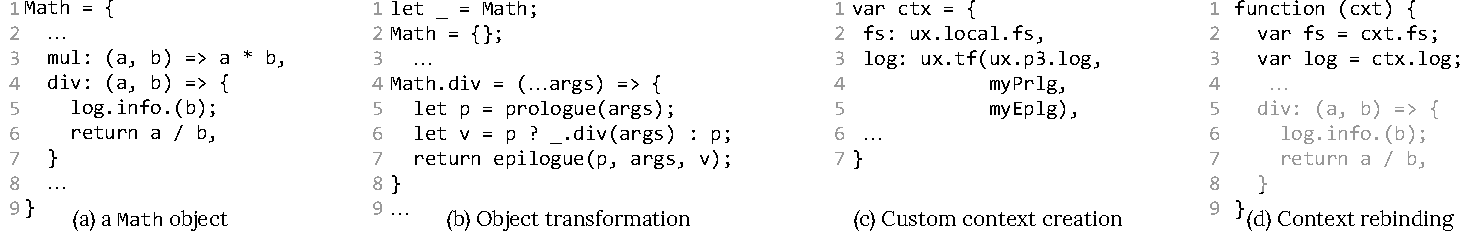
\includegraphics[width=0.99\textwidth]{./figs/lya_ex2.pdf}
\vspace{-2mm}
\caption{
  \textbf{Example transformations.}
   Applying runtime transformations (b) and context rebinding (c, d) on a simple \ttt{Math} object~\cf{impl}.
}
\label{fig:ex2}
\vspace{-4mm}
\end{figure*}

This section details the implementation of \sys for server-side JavaScript (Node.js v8.9.4) in about 1.5K LoC~\sx{impl1},
and the three analyses developed atop \sys~\sx{impl2}.
% We start with the internals of \sys's implementation, and then describe
The differences between JavaScript and other languages are left for \S\ref{reqs}. 
% How other environments diverge from JavaScript is discussed in a later section~\sx{reqs}.

The aforementioned \sys design can be implemented in either of two ways.
The first is to implement \sys as a modified version of the runtime, in which several stages of its library-loading facility have been augmented in-place. % with the techniques described earlier.
The second approach is to implement \sys as a third-party library (\eg the \ttt{lya} package) available by the language's package manager.
% 
With both approaches, \sys feels to users as a backward-compatible, drop-in replacement of Node's module system.
We went with the second approach, as looser coupling seems to have several benefits:
  it does not force \sys's users to have a Node copy only for running analyses;
  it removes \sys's developers from the critical path of updates between the Node developers and its users; 
  and it simplifies \sys's comparison with vanilla Node (both in terms of performance and correctness).
The primary drawback was missing a few opportunities for lowering runtime-performance and development-effort.

\subsection{System Implementation}
\label{impl1}


Node's module system is implemented entirely in JavaScript, exposing a library-local \ttt{require} function for importing modules.
Loading a fresh module % with \ttt{require("foo")}
  corresponds to the following five stages, all of which are augmented by \sys:
(R) Resolution: identify the file to which the module specified corresponds, locate it in the file-system, and assign its absolute path as a module identifier.
(L) Loading: depending on the file type, identify the corresponding loader---\eg V8 compiler for \ttt{js}, \ttt{JSON.parse} for \ttt{json} \etc
(W) Wrapping: wrap the module so that local names do not escape the module's scope and Node's module-local names get resolved.
(E) Evaluation: evaluate the wrapped module in the current context, so that global names and top-level objects get resolved correctly.
(C) Caching: add the module to a handful of module-related caches, for purposes of consistency and performance.

% The resolution algorithm is somewhat convoluted, because it depends on several different facts (including the type of the file requested, whether it is a globally installed, whether it is a directory \etc).
% It does not require any \sys support beyond copying the directory that contains the source code of the all the modules onto the remote host.
% \sys interposes on all of these steps to facilitate transformations.
\sys augments all of these steps.
Interposing on resolution (R) makes the module identifier available to \sys without affecting the (incredibly convoluted!) module resolution algorithm.
If the module's type corresponds to a module that can be analyzed by \sys, \sys fetches the corresponding analysis during loading (L).
Wrapping (W) and evaluation (E) are where \sys transforms the module boundary.
\sys replaces Node's wrapper function to pass an additional argument, the modified context \ttt{CTX}.
\sys comes with a hard-coded list of variable names available to the code of a module, such as \ttt{require} and \ttt{Array};
  the list contains about 150 entries and corresponds to the specific versions of EcmaScript and Node.
Identifying names coming from EcmaScript was relatively easy, as the standard makes them explicit.
Node's global names are described at various parts of the documentation, but library-local names required close inspection of Node's internals; fortunately, they were only five names.

% Before a module's code is evaluated, the Node.js module loader wraps the module so that
%   (i) it keeps top-level variables (declared with \ttt{var}, \ttt{const} or \ttt{let}) scoped to the module rather than the global object; and
%   (ii) it provides some global-looking variables that are actually specific to the module, such as the \ttt{module} and \ttt{exports} objects that the implementor can use to export values from the module and convenience variables---such as \ttt{\_\_filename} and \ttt{\_\_dirname}  containing the module's absolute filename and directory path, respectively.
% True globals remaining are
%   (i) the global objects as defined by the EcmaScript standard (\eg \ttt{Object}, \ttt{Function}, \ttt{Math}); and
%   (ii) Node.js-specific globals (\eg \ttt{console}, \ttt{process}, \ttt{timer}).
% These globals require further interposition.

We found it useful to add an option for white- and black-listing libraries.
The configuration object accepts \ttt{only} and \ttt{not} expressions that indicate whether a module identifier will be part of the analysis.
These expressions contain sets of regular expressions, pattern-matching against module identifiers, which in Node are represented as absolute file-system paths.
Originally intended as an aid to \sys's development and debugging, this option proved useful enough for writing the three analyses that we decided to expose it to \sys's users.
Examples of its use include blacklisting built-in libraries or white-listing only the library imported most recently.

Fig.~\ref{fig:ex2} exemplifies \sys's transformation techniques in the context of JavaScript.
\sys traverses a \ttt{Math} object, replaces functions such as \ttt{div} with wrappers, creates a modified version of the surrounding context, and binds it to the library.


\subsection{Individual Analyses}
\label{impl2}

Individual analysis are implemented using a set of templates that provide initial constructs.
\sys offers a small utility library to reduce boilerplate code for pattern-matching on types.
Individual analyses are about 60 lines of code, but a significant part of this code is common across them.

As the three analyses are too complex to include in the paper, we present here a trivial analysis---one that counts all accesses to global variables from a module \ttt{serial}:

\begin{lstlisting}
let fs = require("fs");
let count = {};
forevery.global.in(/serial/).do({
  pre: (name, path, _) => {
    let o = resolve(name, path);
    count[o] = count[o]?  count[o] + 1 : 1;
  } });
process.on("exit", () => {
  fs.writeFileSync("acl.json",
                   "utf-8",
                   JSON.stringify(count)); });
\end{lstlisting}

\noindent
\sys-provided \ttt{forevery} generates sets of names succinctly.
The \ttt{in} field is a method that takes a regular expression matching module identifiers.
If not empty, \ttt{pre} and \ttt{post} hooks are called before and after each access of the elements specified in the set.
Finally, \ttt{resolve} is a method for traversing an object given a path within that object.
Upon program exit, the results are written to disk, all using the expected Node APIs.

\heading{Security Analysis}
To address the security concerns of third-party libraries, we developed an on-off policy that analyzes accesses for every library-to-library combination.
The analysis treats built-in libraries and global variables as modules,
% and generates a list of permissions for each of their fields.
and develops a permission-like model where individual fields are governed by permission sets containing combinations of on and off permissions.
At the start of the analysis all permissions are set to off (\ie default-deny), and gradually turn on based on the accesses they detect.
Example accesses include:
 (i) reading a value, including assigning it to a variable and passing it around to other modules;
 (ii) modifying or deleting a value; and
 (iii)  executing a value---\eg a function or a method---or invoking a constructor (usually prefixed by \ttt{new}).

The resulting permission sets are organized as collections of maps, one per library, indexed by object-paths---\eg \ttt{require("Math").add: ON}.
% that correspond to values of other modules or global-like language names.

\heading{Performance Diagnosis}
We developed a profiling analysis that operates at two levels:
 (i) module-boundary wrappers that collect profiling statistics for calls between modules by wrapping module interfaces; and
 (ii) an aggregator function that collects statistics from all boundary wrappers and generates a model of library load under the current workload.

Boundary wrappers operate at a higher-frequency intervals than the aggregator, which operates on summaries.
Their analysis focuses on function calls, skipping all other direct field accesses.
Functions are wrapped with prologue and epilogue wrappers that record statistics from the Node.js runtime---for now, a frequency counter and a timer between prologue-to-epilogue invocations.
% Many statistics are available by the Node.js runtime, including memory and garbage-collection statistics, 
Boundary wrappers summarize these statistics by periodically sending a windowed, weighted average of call latencies to the aggregator function.

% Wrappers record statistics about the their encapsulated functions as well as queue characteristics of outstanding calls.
% The wrapper epilogue has access to several raw metrics related to profiling (Tab.~\ref{tab:metrics}).
% These metrics are viewed as a windowed average that priori 

Interestingly, profiling functions at the boundary cannot ``see through'' libraries to correctly attribute load among a library and its dependencies.
For example, a boundary wrapper \ttt{A} of a dependency tree \ttt{A}$\rightarrow$\ttt{B}$\rightarrow$\ttt{C} does not know how much of the latency comes from \ttt{B}.
Fortunately, the aggregator understands the dependency structure and can approximate how much of the latency comes from each module.
% Such a approximation is more complicated than a simple subtraction, as a module may invoke interfaces from multiple modules at the same time.
% Having an analysis fragment per library consumer, however, alleviates much of the problem.

\heading{Type Invariant Discovery}
To infer type invariants for serialization specifications, we based our analysis on a simple type system modeled after the simply-typed lambda calculus augmented with:
  (i) unions (sum types), such as \ttt{string | number}, 
  (ii) JavaScript-specific types such as \ttt{null}, \ttt{NaN}, or \ttt{undefined}, and
  (iii) a \ttt{native} type for values that cannot be serialized, such as \ttt{console.log}.
Support for union types is useful for when our analysis witnesses variables holding values of different types---although, in practice,  programs tend to make calls of the same type across their entire lifetime~\cite{daikon}.

Our implementation also uses a base set of JavaScript types and rules to deconstruct complex types into their elementary building blocks.
% Knowing how to deconstruct a type to its structural primitives allows walking values---
For example, it unpacks a type \ttt{user} into two \ttt{string}s (first and last name) and a \ttt{number} (age).
% To achieve this, the analysis makes use of introspection to identify 

% leftpad: (string | number) -> number -> (string | null) -> string 

% \subsection{Limitations}
% A limitation of our implementation is that it cannot analyze the library importing \sys---usually, the top-level program entry-point equivalent to \ttt{main}.
% This is because \sys cannot transform the context of that file
% As a result, \sys as-is cannot be applied to, say, to analyze single-file programs---a common pattern in scripting languages often used for quick-and-dirty tasks.
% The simplest workaround here is to create an auxiliary file that imports \sys, and then import the single-file script (which, in most scripting languages would invoke it).

\section{Evaluation}
\label{eval}

At a high level, we are interested in three main questions:

\begin{itemize}
  \item \textbf{Q1} Given its coarse granularity, is \sys useful?
    We answer this question in \S\ref{bg}, which shows three case-study multi-module analyses with practical implications.
    \sys operates at the right level of abstraction for answering important questions raised by today's software engineering practices.

  \item \textbf{Q2} Is it usable?
     We answer this question in \S\ref{impl}, by implementing these and other analyses.
    \sys operates as a library around unmodified runtime environments, does not require investment in a new language, and leads to analysis expressions that are comparable to conventional frameworks.
    % Analyses expressed in \sys are about 4$\times$ smaller than equivalent analyses written for a heavy-weight instrumentation framework.

  \item \textbf{Q3} How does it perform? We answer this question here.
  For the most libraries, \sys overheads are under 5\%~\sx{meso}.
  \sys is over an order-of-magnitude faster than Jalangi, a state-of-the-art dynamic analysis framework~\sx{meso}.
  By executing on unmodified runtimes, \sys has significantly better compatibility:
    to execute, Jalangi requires significant library modifications~\sx{meso}.
  \sys scales to three large applications with hundreds of libraries while interposing on several thousands of objects~\sx{macro}.
    Most of the overheads ($>95\%$)come from tracking global variables, but loading-time wrapping and runtime interposition overheads are negligible~\sx{micro}
  % The majority of the overheads come from the use of \ttt{with}, a 

\end{itemize}

% \sys's  development achieves goals \textbf{G1--3}~\sx{goals}, demonstrating that it is indeed feasible to build a framework that 
%   operates as a library around an existing runtime,
%   does not require learning a new language, and 
%   gets meaningful information while operating only at library boundaries.
% % Despite the fact that it operates at coarser granularity, as shown earlier~\sx{impl} \sys can express analyses that generate results useful in several practical scenarios.
% In this section, we report on \sys's performance characteristics:
% % At a high level, we are interested in three questions:
%   (i) the overheads of its underlying building blocks;
%   (ii) \sys on real libraries, and how they compare to a production-grade dynamic analysis; and
%   (iii) \sys's behavior on realistic  multi-library applications.
% % For the first question, we use  synthetic micro-benchmarks that built to stress key elements of the system and confirm it works correctly~\sx{micro}.
% % For the second question, we use real libraries and compare them with an analysis written in Jalangi~\sx{meso}.
% % For the third question, we use a combination of real applications~\sx{macro}.


Experiments were conducted on a modest server with 4GB of memory and 2 Intel Core2 Duo E8600 CPUs clocked at 3.33GHz.
In terms of software, we used Docker version 18.09.7 running a minimal Ubuntu 14.04.6, Jalangi v2, Node.js v8.9.4 (bundled with V8 v6.1.534.50, LibUV v1.15.0, and npm v6.4.1), all atop a Debian Linux with kernel v4.4.0-134.
All times reported are in \textbf{ms}, averaged over 1K runs;
  \textbf{SA}, \textbf{PD}, and \textbf{TID} respectively stand for security analysis, performance diagnosis, and type invariant discovery.
  

% \begin{table}[t]
% \center
% \footnotesize
% \setlength\tabcolsep{3pt}
% \caption{
%   \footnotesize{
%     \textbf{Analysis results for the largest libraries.}.
%     The table shows the overheads of applying the three analyses to the test suites of eight libraries. % (with Minimist involving five test cases).
%   }
% }
% \begin{tabular*}{\columnwidth}{l @{\extracolsep{\fill}} lll l}
% \toprule
%                                & Base   &  SA   & PD     &   TID   \\
% \midrule
% Classnames~\cite{classnames}   &  2.72  & 6.62  &  6.61  &  6.10   \\
% Debug~\cite{debug}             & 31.39  & 33.54 &  33.94 &  33.96  \\
% Minimist~\cite{minimist}       &        &       &        &         \\
% ~~~-t1                         & 31.46  & 60.13 &  60.00 &  56.62  \\
% ~~~-t2                         & 29.35  & 56.30 &  53.98 &  53.17  \\
% ~~~-t3                         & 30.34  & 59.13 &  55.76 &  55.34  \\
% ~~~-t4                         & 30.04  & 56.40 &  53.68 &  53.27  \\
% ~~~-t5                         & 30.24  & 58.17 &  55.07 &  54.76  \\
% Moment~\cite{moment}           & 31.73  & 48.04 &  49.23 &  44.95  \\
% yargs~\cite{yargs}             & 14.59  & 15.68 &  15.49 &  15.54  \\
% chalk~\cite{chalk}             & 17.37  & 24.42 &  26.01 &  26.32  \\
% colorette~\cite{colorette}     & 08.10  & 13.85 &  13.41 &  13.16  \\
% mkdirp~\cite{mkdirp}           & 116.37 & 1959.52 & 1392.64 & 1252 \\
% \bottomrule
% \end{tabular*}
% \label{tab:meso}
% \vspace{-5mm}
% \end{table}



\subsection{Single-Library Benchmarks}
\label{meso}

\begin{figure*}[t]
  \centering
   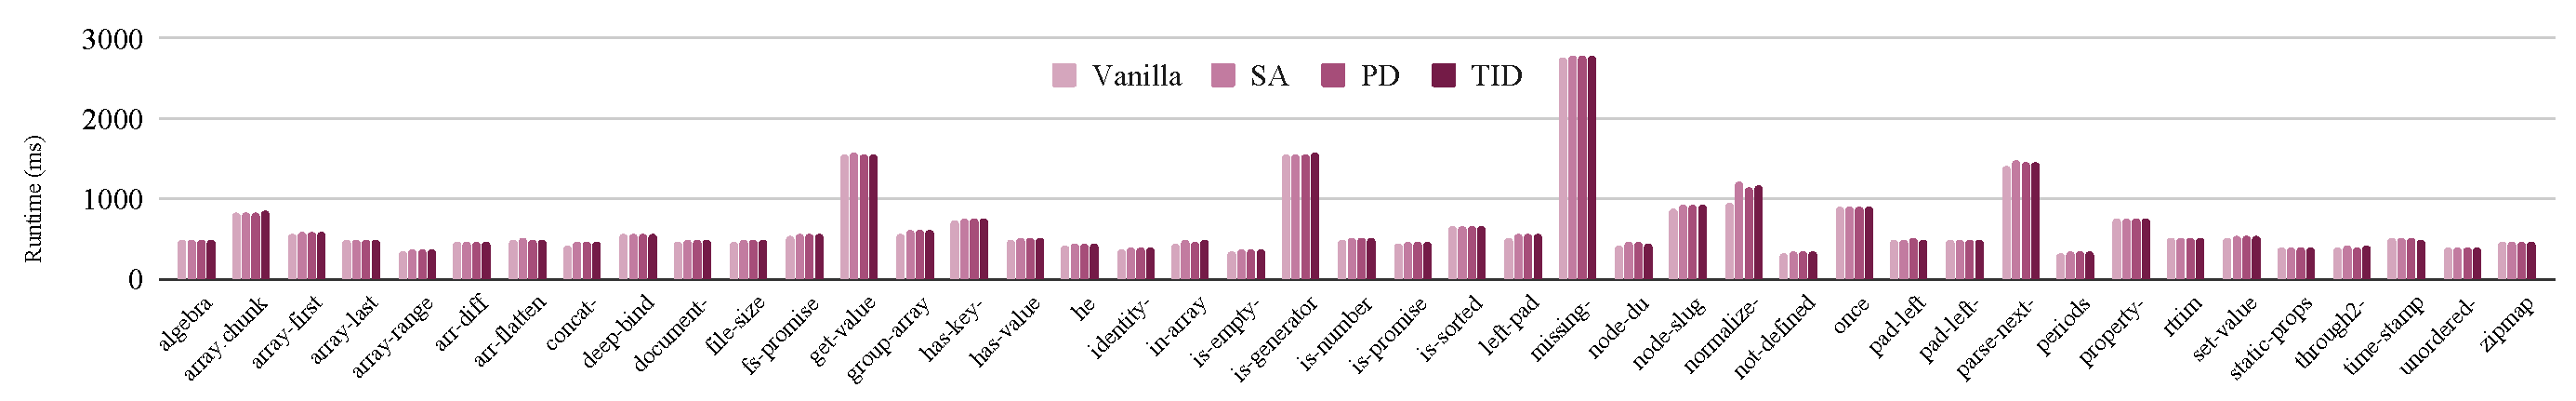
\includegraphics[width=\textwidth]{./figs/micro-packages.pdf}
  \caption{
    \textbf{Runtime overhead.}
    The plot shows the runtime overhead of the three analyses for 50 libraries against normal (vanilla) execution~\cf{meso}.
  }
  \label{fig:micro-packages}
  \vspace{-3mm}
\end{figure*}

To understand \sys's performance characteristics at the level of individual modules, we performed two experiments.

\heading{\sys on Popular Libraries}
For the first experiment, we evaluate \sys on 50 JavaScript packages from the npm ecosystem.
These libraries are highly popular, averaging 4.8M weekly downloads (total: 227M) and are depended upon by about 656 other packages or applications on average (total: 30K).
% More results about the javascript packages here: https://docs.google.com/spreadsheets/d/18xKjCgj1phODbNi6_IT-y3vP3oVaaY5oA-Wux2avvGY/edit#gid=2071117281
These libraries are relatively small---adhering to known ecosystem trends~\cite{npmstudy:19}---simplifying compatibility inspection.

Each library was run against the test suite provided by its nominal developers, via \ttt{npm test}.
As these libraries are quite popular, they have received significant investment in their testing infrastructure, resulting into two main benefits for \sys's evaluation:
  (i) different tests stress different parts of the library and corresponding analysis primitives;
  (ii) even if most applications that import these libraries use only a fraction of their functionality, tests still cover the majority of provided functionality---\eg we observed test suites that were $10\times$ the size of the corresponding library.  

Fig.~\ref{fig:micro-packages} shows the performance overhead of applying \sys on these libraries.
Overheads report on running each library's entire test suite under the three analyses and comparing against the non-\sys version.
On average, \sys's analyses add about 3.3ms per library causing 1.93\% slowdown;
  relative overheads between analyses are negligible (avg: $<$0.1ms).
For the largest of these libraries, we perform a lighter global-access analysis (not shown in Fig.~\ref{fig:micro-packages}).
This is slightly faster, adding a 3.2ms causing a 1.62\% slowdown.
We zoom into the sources of these overheads later~\sx{micro}.

\heading{\sys vs. Jalangi}
For the second experiment, we compare the performance of \sys to that of Jalangi.
Jalangi is a popular dynamic analysis framework for JavaScript, providing fine-grained instrumentation by executing on a custom interpreter.
We note our use of Jalangi's v2.2.5 version:
  the v2 branch improves significantly over the performance of the original framework~\cite{jalangi}, as it eschews record/replay capabilities.

In terms of programs, we use Jalangi's extensive test suite within a Jalangi-provided docker container~\cite{jaladocker}
(For these experiments, \sys is also run in the same container.)
This is not entirely by choice:
  Jalangi's interaction with the bare-bones libraries was hitting EcmaScript 6 parsing challenges, further complicated by \ttt{npm test} (which is an external program outside Node, but tightly coupled with it).
Contrary to Jalangi, \sys executes all programs, demonstrating the compatibility benefits of operating on an unmodified runtime.

% FIXME OSDI
% This is an important practical difference with \sys approach:
%   if \sys does not understand, it will simply not wrap it---deferring silently to the default semantics implemented by the runtime rather than

In terms of analysis, both systems are configured to perform dynamic frequency analysis of accesses to global variables.
The analysis is a common denominator between \sys and Jalangi, designed and implemented from scratch to ensure a % fair and 
  meaningful comparison between the two frameworks.
Such analyses are useful for understanding program components interact with global state---\eg for generating remote-procedure stubs or scaling out functional components~\cite{ignis}.

Fig.~\ref{fig:meso} presents the comparison between \sys and Jalangi.
The core of the analysis requires a few lines, but expressing it in \sys requires 4$\times$ fewer lines of code.
% the effort of employing \sys as a library was also significantly lower than that of Jalangi2, for which we relied on a Docker container to simplify the framework's setup.
The performance results show that \sys performs better than Jalangi, at times by a significant margin (\ie more than 10$\times$ for 13 benchmarks).

Implemented as a custom interpreter, Jalangi exists at a different point in the trade-off space than \sys.
On the one hand, it is significantly more fine-grained than \sys, capable of expressing and executing analyses at the granularity of individual expressions.
On the other hand, it results in significantly higher incompatibility and runtime overhead---even when the analysis does not make use of its features.

\begin{figure*}[t]
  \centering
   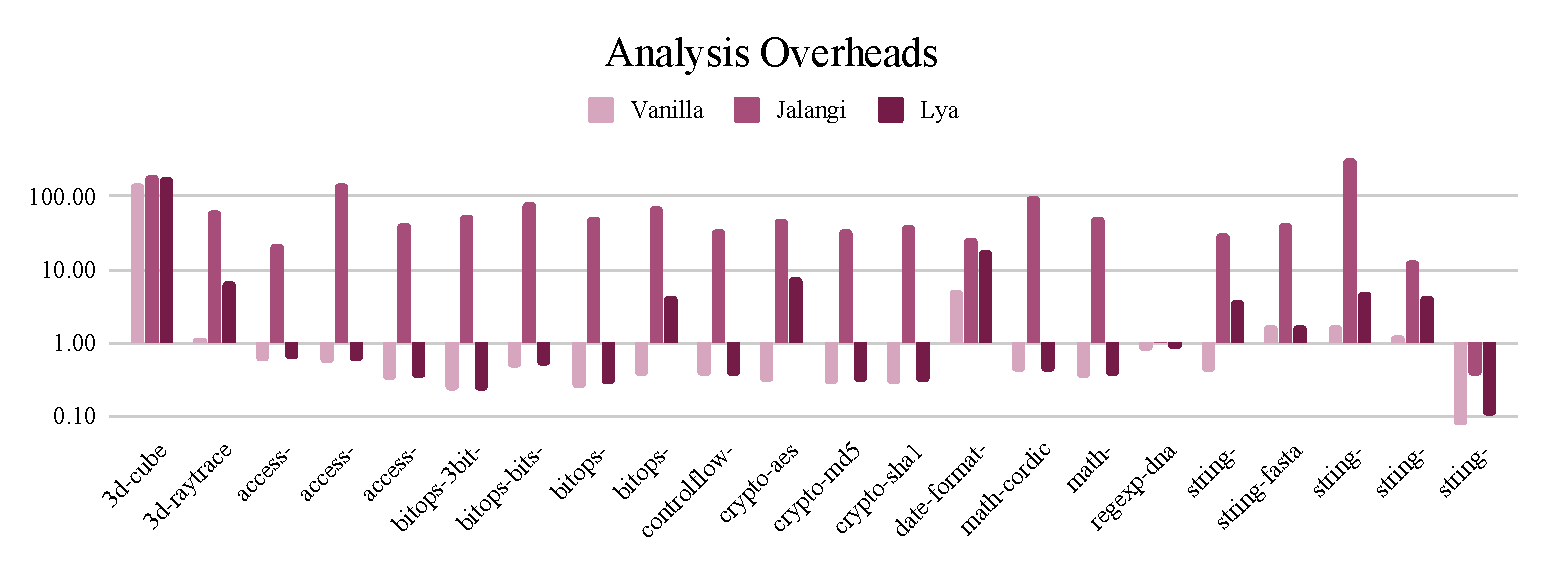
\includegraphics[width=\textwidth]{./figs/meso.pdf}
  \caption{
    \textbf{\sys vs. Jalangi.}
    The plot compares single-library programs taken from Jalangi between three setups:
		(i) Vanilla JavaScript, (ii) global-use analysis with Jalangi, (iii) global-use analysis with \sys.
    Global-use analysis is a simple analysis that tracks accesses of global variables in the program~\cf{meso}.
  }
  \label{fig:meso}
  \vspace{-3mm}
\end{figure*}


\subsection{Application Benchmarks}
\label{macro}

\begin{table}[b]
\center
\footnotesize
\setlength\tabcolsep{3pt}
\caption{
  \footnotesize{
    \textbf{Applying \sys to three large applications}.
    The table shows the characteristics and runtime overheads of applying the three analyses to three large applications~\cf{macro}.
  }
}
\begin{tabular*}{\columnwidth}{l @{\extracolsep{\fill}} ccc}
\toprule
                                     & KoaBlog~\cite{koa}    & Moeda~\cite{moeda}   &  Term/zr~\cite{terminalizer} \\
\midrule
Structure                            &                   &                      &              \\
~~Size (MB)                          & 41                &  29                  &   262        \\
~~Code Size (KLoC)                   & 127               &  79                  &   39         \\
~~Top-level Modules, statically      &  24               &  7                   &    33         \\
~~Total Modules, statically (npm)    &  432              &  260                 &    1084       \\
~~Total Modules, dynamically (\sys)  &  1507             &   729                &     2355      \\
%                                     &                   &                      &              \\
Performance (s)                      &                   &                      &              \\
~~Baseline                           &  0.97             &  1.27                &    0.754      \\
~~Security Analysis                  &  1.48             &  2.00                &    3.346      \\
~~Performance Diagnosis              &  1.30             &  2.684               &    2.684      \\
~~Type Invariant Discovery           &  1.32             &  2.036               &    2.615      \\     
\bottomrule
\end{tabular*}
\label{tab:macro}
\vspace{-5mm}
\end{table}


We apply \sys on three large applications:
  KoaBlog~\cite{koa}, a minimal blogging platform built on the Koa framework;
  Moeda~\cite{moeda}, a command-line currency converter that, among other features, uses online currency exchange rates; and
  Terminalizer~\cite{terminalizer}, an application for recording terminal sessions to generate animated gif images and shareable web-player links.
These applications are highly popular, with Koa and Terminalizer having 28.3K and 8.7K GitHub stars respectively.
Their structural and performance characteristics are shown in Tab.~\ref{tab:macro}.

The differences between the number of sub-modules detected statically (by \ttt{npm ls}) and the ones observed by \sys are due to a few reasons.
One is that \sys does not report accesses if a library is not accessed at runtime, whereas \ttt{npm} traverses and reports on the entire dependency structure.
\sys analyzes modules that are part of the standard library (some of which have themselves internal dependencies),  not shown by \ttt{npm}.
Finally, \sys generates several different return wrapped objects for the same libraries~\sx{three}.

Applying \sys to these applications generates analysis results that are 9--132$\times$ larger than the ones for single libraries.
However, the performance of analyzed code is on average still within 2--3$\times$ over the baseline performance.
The size of the resulting JSON files raises the challenge of analysis interpretability---just by running Terminalizer with \ttt{--help} returns more than 6K fragments from several (hundreds of) libraries.
Custom \ttt{onExit} analysis routines post-process \sys's results to compress by module name---\ie squashing duplicate reports by human-readable name, not file-system module identifier.
This can affect the results of multiple imports with the same name at different parts of the tree that would indeed correspond to different libraries.
% For example, importing two different versions of a library at two different parts of the dependency tree will result in to two different with the same name.
We also squash cache entries that correspond to one module imported by multiple modules, which would create separate entries in \sys's augmented cache, but results in a single count for Tab.~\ref{macro} (for \sys's treatment of the module cache, see~\S\ref{three}).
Confirming that \sys performs correctly under these scenarios is one part of the motivation behind the synthetic micro-benchmarks shown earlier~\sx{micro}.

\subsection{Micro-benchmarks}
\label{micro}


\sys's micro-benchmarks zoom into \sys's sources of overheads.
The key results are that
  (i) the majority of the overhead comes from the JavaScript's \ttt{with} expression, which \sys uses to wrap the context of libraries;
  (ii) interposition overhead is negligible in practice;
  (iii) while wrapped and accessed fields increase exponentially as a function of depth (as objects have many fields), object explosion quickly plateaus around level four with under 400 fields; and
  (iv) the majority of wrapped and accessed fields come from Node and EcmaScript names rather than imports or global values.

\heading{Sources of Overhead}
To understand the sources of these overheads, we perform a series of micro-benchmarks with tight loops calling several ES-internal libraries without any I/O.
By enabling different parts of \sys, we discover that the primary source of overhead comes from JavaScript's \ttt{with} construct:
  disabling \ttt{with} makes 95\% of the overheads disappear.
The reason \ttt{with} dominates overheads is twofold: it (i) interposes on too many accesses, only a fraction of which are relevant, and (ii) remains significantly unoptimized, since its use is strongly discouraged by the JavaScript standards.


\begin{table}[t]
\center
\footnotesize
\setlength\tabcolsep{3pt}
\caption{
  \footnotesize{
    \textbf{Synthetic Micro-benchmarks}.
		Applying the three analyses on a series of synthetic micro-benchmarks, created to stress different features.
    All timings are in $ms$~\cf{micro}.
  }
}
\begin{tabular*}{\columnwidth}{l @{\extracolsep{\fill}} lll l}
\toprule
	               &   Base    &  SA     & PD      &  TID    \\
\midrule
global  vars     &   0.90    &  4.70   &  4.54   &  4.30   \\
built-in fields  &   1.44    &  6.46   &  6.24   &  5.96   \\
counter          &   3.37    &  6.26   &  6.32   &  5.72   \\
all names        &   7.79    &  13.54  &  13.31  &  12.8   \\
custom delays    &   24661   &  24848  &  24754  &  24760  \\
direct-access    &   4.06    &  7.24   &  7.16   &  6.79   \\
simple-types     &   4.11    &  7.25   &  7.23   &  6.86   \\
cycles           &   4.32    &  8.32   &  8.19   &  7.73   \\
\bottomrule
\end{tabular*}
\label{tab:synthetic}
\vspace{-5mm}
\end{table}


\heading{Interposition Overheads}
Table~\ref{tab:synthetic} depicts the results of the three analyses applied to a subset of the aforementioned synthetic benchmarks.
The first column indicates the focus of the benchmark; not all analysis--benchmark combinations are useful:
  for example, the ``custom-delay'' benchmark features static bottlenecks across its dependency tree but does not involve interesting access patterns.
\sys-induced slowdown is under 2$\times$, except for the first two cases that feature \emph{only} accesses.
Close inspection confirms a correlation to the number of wrapped objects and the frequency of accesses:
  these benchmarks feature artificially tight loops with high-frequency accesses.
Transformation overheads themselves (not in Tab.~\ref{tab:synthetic}) remain under 1ms.

To understand the costs of proxy interposition, we measure the time to access deeply-nested properties of two versions of an object:
  unmodified and proxy-wrapped.
Paths to the properties (\eg \ttt{a.b.c.$\ldots$}) are random but generated prior to running the experiment.
We construct 500MB-sized objects, each with a fanout of 8 fields nested for 12 levels.
The proxy-wrapped version introduces interposition at every level.
Traversing one million 12-edge paths (\ie root to leaves) averages 167.2ms and 595.7ms ($3.5\times$) for the unmodified and proxy-wrapped versions, respectively.
% 
We emphasize that this is an artificially constructed benchmark stressing worst-case overheads nowhere near an normal execution:
  for comparison, the transformation of these objects itself took nearly 16 seconds ($10^3\times$ more than what we saw with real modules).
The takeaway is that \sys-inherent overheads due to interposition are unlikely to be the bottleneck of an analysis;
  what is likely to be is the analysis itself---\eg updating a global aggregator or invoking system-calls to extract timing.

\heading{Analysis Depth}
To understand the effect of depth in practice, Fig.~\ref{fig:objects} presents the number of wrapped object, unique accesses, and total accesses as a function of depth for all 50 libraries~\sx{meso}.
Depth is explained in the previous paragraph:
   it is about how deep \sys traverses references starting starting from the names in scope---\eg the access \ttt{global.obj.x} is two levels deep and \ttt{fs.readFile} is one level deep.

There are a few highlights worth noting.
While the number of objects wrapped by \sys starts growing rapidly, it quickly reaches an average upper bound of 400 (depending on the exact benchmark).
Accesses grow exponentially for the first couple of levels---as objects at levels have multiple fields, many of which are accessed several thousand times---but then stabilize around level 5.
This is because most interfaces follow a mostly-flat format where all methods are defined at the top level or right under.

\begin{figure}
  \centering
  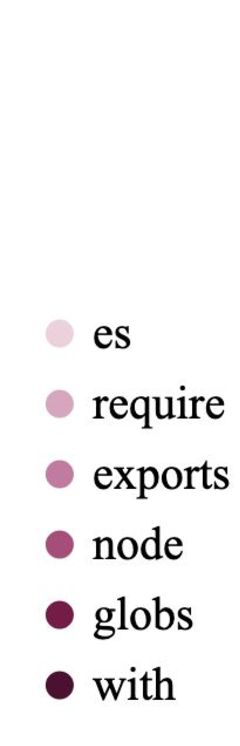
\includegraphics[width=0.05\textwidth]{./figs/lya_donut_index}
  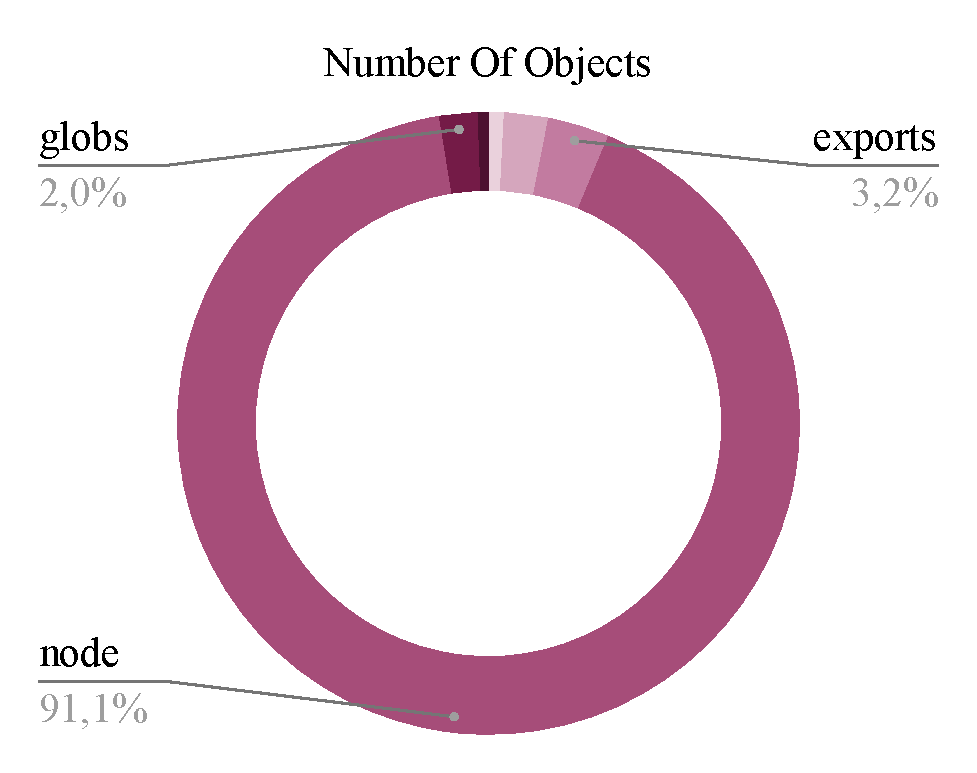
\includegraphics[width=0.20\textwidth]{./figs/lya_ctx_obj}
  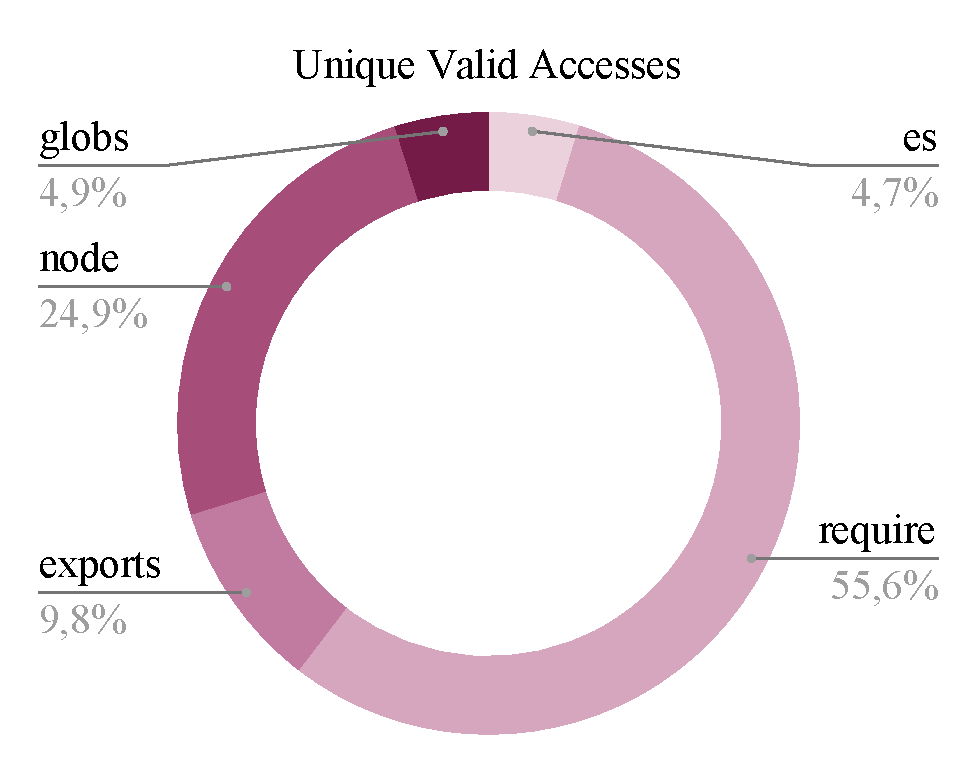
\includegraphics[width=0.20\textwidth]{./figs/lya_ctx_unique_valid}
  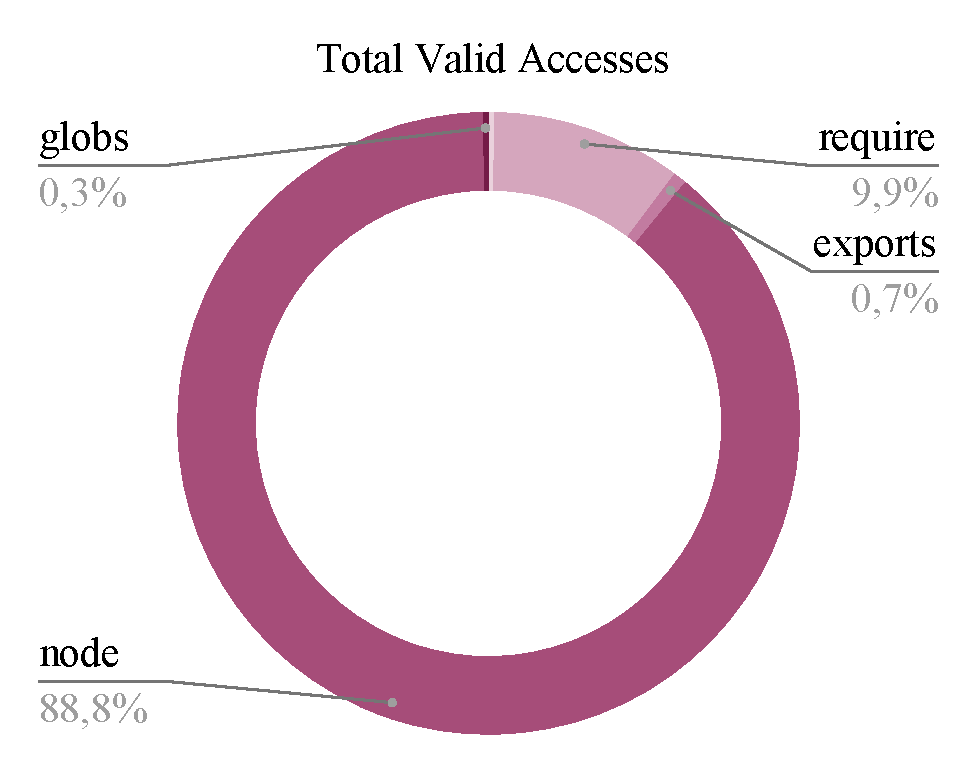
\includegraphics[width=0.20\textwidth]{./figs/lya_ctx_total_valid}
  \caption{
    \textbf{Access characteristics as a function of context.}
    Clockwise from top-left:
    (i) number of \sys wrappers,
    (ii) unique valid accesses (\ie counting each access once),
    (iii) total valid accesses~\cf{micro}.
    \vspace{-4mm}
  }
  \label{fig:objects}
\end{figure}

\heading{Context}
Context refers to the broad source of names that are available in the current scope---ones
  defined by the EcmaScript standard (es), 
  through an explicit import (exports),
  by the Node.js runtime (node), or
  via global variables (globs).
A few names seem globally available but are in fact module-locals (\ttt{require}).
User-defined global variables are not prefixed with \ttt{global} thus requiring special interposition (\ttt{with}).

Fig.~\ref{fig:objects} shows \sys's context characteristics on all 50 libraries~\sx{meso}. % as a function of context.
In terms of the number of objects wrapped, the majority comes from Node (91.1\% of all wrappers).
In terms of unique number of accesses, for both invalid and invalid the majority comes from \ttt{require};
  taking their number into account, valid accesses concentrate on ES and Node, whereas invalid ones concentrate on \ttt{export}s.

\begin{figure}[t]
  \centering
  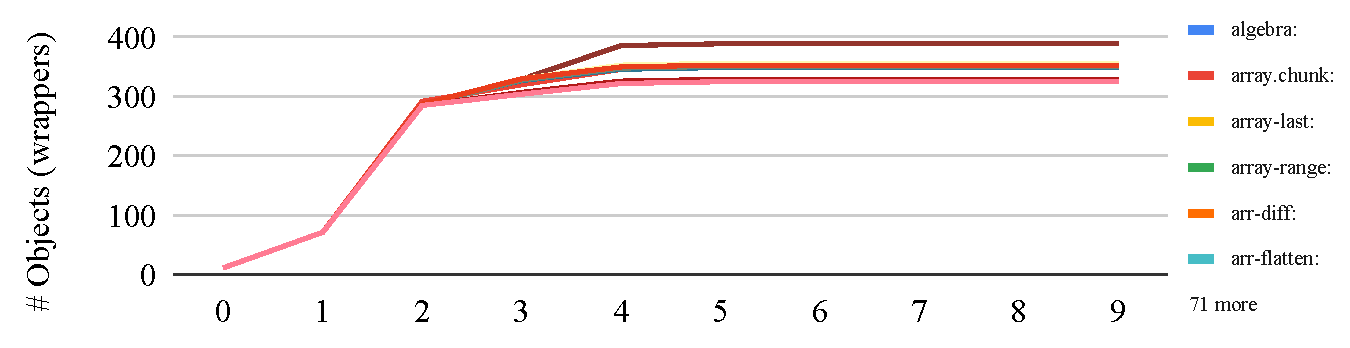
\includegraphics[width=\columnwidth]{./figs/lya_n_obj}
  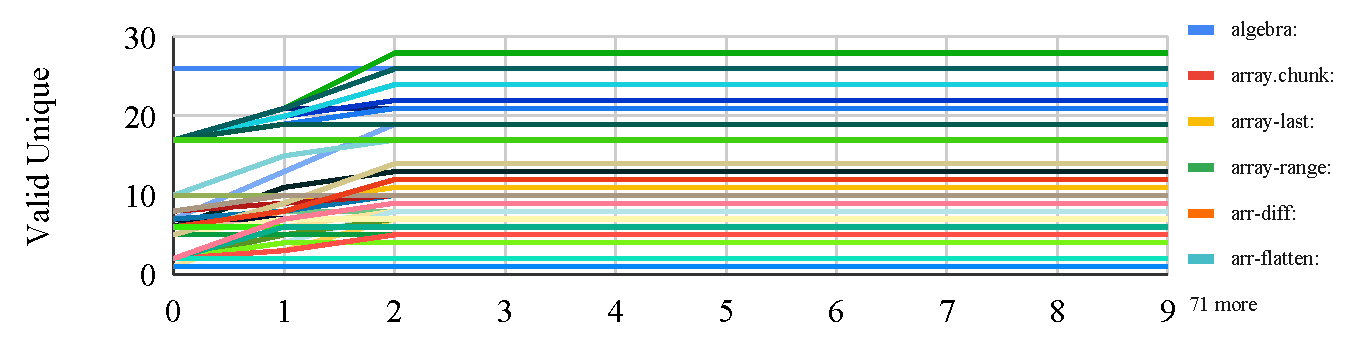
\includegraphics[width=\columnwidth]{./figs/lya_unique_valid}
  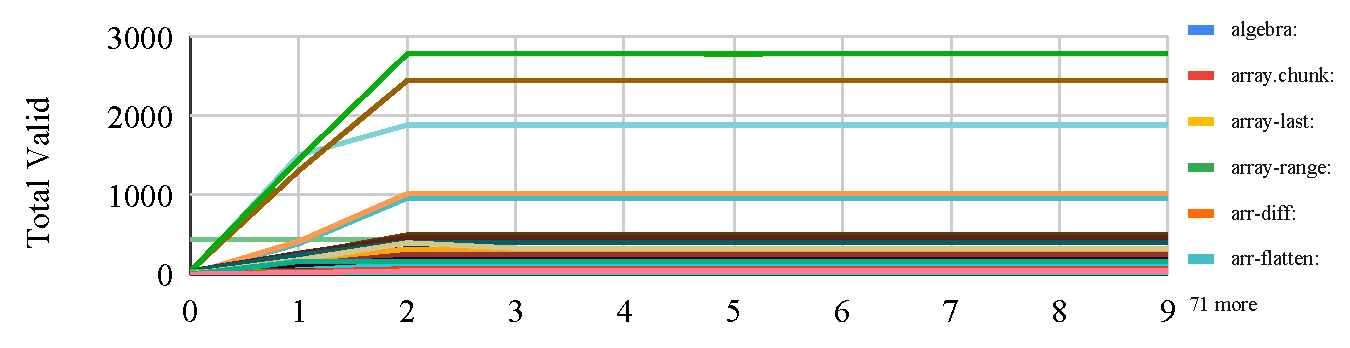
\includegraphics[width=\columnwidth]{./figs/lya_total_valid}
  \caption{
    \textbf{Analysis characteristics as a function of the analysis depth.}
    From the top:
    (i) number of \sys wrappers applied,
    (ii) number of unique accesses (\ie counting each access once),
    (iii) total number of accesses~\cf{micro}.
    \vspace{-5mm}
  }
  \label{fig:objects}
\end{figure}

\section{Discussion}
\label{diss}

This section discusses \sys's minimum requirements~\sx{reqs} and reflects on its strengths and weaknesses~\sx{principles}.

\subsection{Applying \sys to Other Environments}
\label{reqs}

The techniques presented in this paper are applicable to any programming language.
We chose JavaScript % to evaluate the feasibility of our approach,
primarily because
  (i) it boasts the largest collection of libraries~\cite{modulecounts} and
	(ii) we had prior experience developing more sophisticated versions of SA and PD.
We now expand on the requirements for bolting our techniques on other runtime environments.

By operating on library boundaries, \sys uses a few special language features supported by all dynamic programming languages.
First, \sys needs to re-wire the \ttt{import} keyword:
  if it is a function (\eg JavaScript, Scheme, Racket), re-wiring amounts to an overwrite;
  if it is a special non-functional keyword, re-wiring needs to be prefixed by a rewriting pass replacing \ttt{import} with a function (during module loading).
% This is simplified by the fact that the import syntax is trivial.

It also needs the ability to interpose on values and transform their components.
% This is relatively easy in languages that provide meta-programming capabilities.
Dynamic programming languages offer runtime reflection and conveniently expose object accesses as (over-loadable) functions---\eg \ttt{Proxy} objects in JavaScript, metatables in Lua, metaclasses in Python, and direct-accessor meta-programming Ruby.
Compiled languages would apply transformations with static metaprogramming facilities, traversing and transforming objects at compile time.
Examples include templates and macro expansions such as Template Haskell and Rust's macro system.
% Other languages, such as Java and Julia, provide both static and dynamic reflection capabilities, allowing considerable freedom in the choice of implementation.
% Fifth, \sys makes extensive use of interposition which is also available in different programming languages.
% Static programming languages provide different types of support for 

\sys makes extensive use of hash-maps to check for object equality, for cycles during traversal, and for prior wrapping.
Hash-maps are supported by every programming language; many support storing weak references, which avoid affecting object reclamation in garbage-collected environments, and can be created either explicitly (\eg Python) or implicitly by using a ``weak'' structure (\eg JavaScript).
% An additional feature useful in garbage-collected languages would be for these (copies of) references to not affect the reclamation of original objects.
% Languages either support the ability to create such a weak reference from a normal reference (\eg Python's weak references), or provide structures that automatically hold weak versions of these references (\eg JavaScript's Weak Map).

Finally, \sys makes use of variable shadowing to hide the original, unmodified versions of values---a universal feature.\footnote{
  A notable exception is the language CoffeeScript. %, which can mimic the same feature using function scope.
}
% Differences in scoping rules---\ie what the shadowed variable ends up referring to upon execution---do not affect the usefulness of this feature, although we have found lexical scoping easier than dynamic scoping.

It is worth noting that \sys does not require the entire source code of the library to be available.
While this is common in dynamic languages, \sys can operate on language-aware wrappers as is common, for example, with Python wrappers around C libraries.

To conclude, all major languages provide facilities to support a \sys-like framework, albeit with a different level of convenience.
Dynamic languages have features---\eg name (re-)binding, value introspection, dynamic code evaluation, and access interposition---that enable runtime transformations, which conveniently unify module identification with interposition:
  a single function-like operator locates a module, interprets it, and applies transformations before exposing its interface in the caller context.
Static languages have other benefits, such as avoiding the runtime overheads of transformations by applying them at compile-time.
% and type checking could further aid developers by issuing warnings of incompatible privilege settings.


\subsection{When to Use \sys-like Analysis}
\label{principles}
While heavy-weight dynamic analysis provides full visibility into program execution, it may suffer from higher performance overheads, require significant developer effort, or offer results that are too low-level for the problem at hand.

The set of techniques presented in this paper shines at a need for urgency, select online analysis, and a high level of abstraction.
It can help identify quickly the source of a problem by swiftly isolating homegrown code from standard and third-party libraries, by requiring a few lines of analysis-specific code to be inlined, and by leveraging the developer's expertise in their language of choice.
By operating at coarser granularity, using the vanilla optimized runtime, and by toggling parts of the analysis on and off, it provides the ability to perform the analysis online.
Finally, it deconstructs programs only at library boundaries, a naturally coarser granularity that is ideal for certain classes of problems.

\sys's set of techniques is \emph{not appropriate} for monolithic programs or ones written in low-level languages such as C, due to several reasons.
C neither features import/export keywords and runtime code evaluation,
% Dependencies often lack \emph{any} source code.
  nor clear, ``impenetrable'' boundaries like the ones available in memory- and type-safe languages.
C libraries can forge pointers and access arbitrary locations in the program's address space, a feature that breaks a key hypothesis in \sys---namely, that the wrapping mechanism can track a library's full observable behavior.
A final problem is C's inability to traverse and wrap objects;
  due to lack of runtime information about size and structure, it is unclear how to traverse and transform them.\footnote{
  Recent efforts such as C-Strider~\cite{saur2016cstrider} and ptrSplit~\cite{ptrsplit:17} show promise.
}

\section{Related Work}
\label{rw}

The previous section~\sx{principles} offers a theoretical comparison between conventional dynamic analysis and \sys.
This section we turn to a technical comparison of \sys to prior systems.

% \heading{Dynamic Analysis Systems}
There are several dynamic analysis frameworks for JavaScript~\cite{javascript1, javascript2, javascript3, mugshot, jalangi}.
Jalangi~\cite{jalangi} and Mugshot~\cite{mugshot} are the most popular and feature fine-grained code-level instrumentation powerful enough to record and replay entire program executions.
This power comes at a significant inconvenience: % as they need to virtualize the entire execution environment.
  they incur 2--3 order-of-magnitude slowdown and are not embeddable in a runtime-agnostic manner.
% source-code-level rewriting every expression corresponding to a profiling event in the original program needs is resolves to a profiling function call.
These features are antithetical to \sys, which leverages basic programming-language primitives to insert high-performance analysis hooks completely transparently to the runtime environment.

NodeProf~\cite{javascript3} is a fine-grained dynamic analysis % atop Truffle~\cite{} and running on top of Graal.js~\cite{graal}, a Node.js-compatible runtime.
  standing at a different point in the analysis design space---more powerful than \sys, but with a significantly higher effort to use.
It instruments a program's AST (rather than the code) statically, % making it easier to maintain compared to source changes but
  limiting the use of dynamic features, assuming knowledge of the underlying Graal~\cite{graal} and Truffle~\cite{truffle} APIs, and requiring recompilation of the Java hooks.
% Different from \sys, it leverages AST extraction and manipulation to build, which is not available in many languages and may be limit by dynamic features such as reflection and JITing.
Nevertheless, some of NodeProf's goals are similar to \sys such as lowering overheads and toggling analysis during execution.
%FIXME: Lya is also limited (i) by dynamic features such as reflection, because they're gonna hit the wrapper and (ii) the equality and other primitive operators

The Aran sketch~\cite{javascript1} proposes proxy-based analysis coupled with JavaScript's unusual \ttt{with} primitive for wrapping custom contexts.
\sys works at the module boundaries, a potentially coarser granularity, without any unusual language constructs.

%% JSConTest2~\cite{javascript2} is a dynamic \emph{access} analysis framework;
%% \fixme{Rather than extracting accesses, it arms developers with the ability to write access control contracts (\ie executable partial specifications)}.
%% This capability is complimentary to \sys's security analysis model~\sx{examples}, illustrating a need for a general-purpose online analysis framework.
%% % \ie their analysis can be implemented on top of \sys with significantly less effort.
%% % build around proxies.

JavaScript is related to WebAssembly, a standardized subset of JavaScript target designed to serve as a compilation target.
The first dynamic analysis framework for WebAssembly, Wasabi~\cite{wasabi}, shares some of \sys' goals---\eg low-effort analysis and API for observation rather than manipulation.
% Wasabi is also programmable in JavaScript (which, however, is not its target language), a similarity to \sys that is mostly accidental:
%   Wasabi needs to be provide a high-level analysis scripting interface and chose JavaScript;
%   whereas \sys's partial goal is supporting analysis in the same language as the program~\sx{goals}. % ---that is, \sys implemented for Python would be using Python abstractions.
Contrary to \sys, Wasabi instruments binaries statically, \ie ahead-of-time, and aims for heavyweight instrumentation.

\sys has some resemblance to dynamic instrumentation frameworks~\cite{pin, valgrind, disl, roadrunner}.
These wrap basic blocks of a program incrementally and right before execution, similar in vein to how \sys wraps libraries.
% Pin~\cite{pin} and Valgrind~\cite{valgrind} translate basic blocks of the program just before their execution;
%   \sys starts by wrapping a library during import, adding a small overhead on its loading time.
However, they operate at a much lower level (binary) than \sys, are much more detailed and heavy-weight, and are usually not available to high-level languages as a language-aware library.

Aspect-oriented programming (AOP) is a programming model where program points map to actions taken at these points~\cite{aop}.
A part of \sys is genetically related to AOP, drawing from proxies, wrappers, mirrors and other related mechanisms up to  metaobjects~\cite{metaobject}.
While aspects are more powerful than \sys's localized transformations, adding support for them in a language is not trivial:
  for example, AspectJ and AspectC++, while extensions of popular languages, require modifications to the original language and/or runtime system.
\sys operates on a completely unmodified language and runtime environment.
% Key ingredients of \sys's approach include variable shadowing, runtime loading, 

% \sys piggy-backs on a common  mechanism of existing (dynamic) languages---runtime module loading---to enable dynamic analysis.
% More generally AOP is related to metaobjects~\cite{metaobject}, objects that manipulate object structure, and which enable a program to access to its own internal structure, including rewriting itself as it executes.
% While \sys uses metaobjects to traverse, understand, wrap, and rewrite interfaces, it shields developers from building the required metaobject infrastructure.
% self element

\sys draws inspiration directly from program fracture and recombination (PFR)~\cite{fracture1, fracture3}, a line of work less tied to program analysis and more towards program synthesis and automated patch generation.
PFR breaks up multiple programs into many components with the goal of exchanging functionality between donor-donee pairs of programs.
Contrary to PFR, \sys operates on single programs, avoids breaking semantics, and leverages the existence of components with (mostly) explicit boundaries in the guise of libraries or modules.

\section{Conclusion}
\label{end}

Recent trends in software engineering have led to unprecedented levels of third-party code (re-)use.
We present \sys, a novel library-oriented dynamic analysis framework for dismantling, analyzing, and reassembling programs by combining name shadowing, context wrapping, and transformation of the underlying dependency graph.
% Contrary to heavy-weight dynamic analysis, \sys lowers developer effort in writing and deploying analysis, improves runtime performance, and operates at a high level of abstraction.
\sys delivers better performance  than conventional analysis systems, improved compatibility, and support for a range of dynamic analyses.

% \sys is  available as an open-source library for experimentation with other applications and analyses.

% \subsection*{Acknowledgments}
% 
% We thank Ben Karel, Jeff Perkins, and the MIT PAC group for their valuable thoughts. 
% Much of \sys's design was informed through interactions with the community---we are particularly thankful to Isaac Z. Schlueter and CJ Silverio from npm and Daniel Katz, Petros Efstathopoulos, Kevin Roundy, and Daniel Marino from Symantec/NortonLifeLock Research Group.
% This work was partly supported by DARPA contract no. HR00112020013 (ALRSCC).

\bibliographystyle{plain}
\bibliography{bib}

\end{document}

%%  LocalWords:  endnotes includegraphics fread ptr nobj noindent
%%  LocalWords:  pdflatex acks
